\chapter{Axiome der Wahrscheinlichkeitstheorie}
$\Omega$ = Menge aller Ausgänge eines Zufallsexperiments\medskip\\
Ereignisse := Teilmengen von $\Omega$\medskip\\
$\mathcal{P}(\Omega)$ = Menge aller Ereignisse = Potenzmenge von $\Omega$\\ $\#\mathcal{P}(\Omega)=2^{\#\Omega}$\medskip\\
Wahrscheinlichkeit ist eine Funktion $\mathds{P}:\mathcal{P}(\Omega) \rightarrow [0,1], A \mapsto \mathds{P}[A] $ mit 
\begin{itemize}
	\item $\mathds{P}[A_1\cup A_2\cup...]=\mathds{P}[A_1]+\mathds{P}[A_2]+...$\\
	$\forall A_1, A_2,... \subset \Omega $ mit $A_i \cap A_j = \emptyset$ $\forall i \neq j$
	\item $\mathds{P}[\Omega]=1$
\end{itemize}
\section{Eigenschaften von $\mathds{P}$}
\begin{enumerate}
	\item $\mathds{P}[\emptyset]=0$
	\item $\forall A_1,...,A_n \subset \Omega $ mit $A_i \cap A_j = \emptyset \quad \forall i \neq j$\\
	$\mathds{P}[A_1\cup,...,\cup A_n] = \mathds{P}[A_1]+...+\mathds{P}[A_n]$\medskip\\
	\textbf{Spezialfall}: Für A,B $\subset \Omega$ mit A $\cap B = \emptyset$\\gilt 
	$\mathds{P}[A\cup B] = \mathds{P}[A] + \mathds{P}[B]$
	\item $\forall A \in \Omega \quad \mathds{P}[A^C]=1-\mathds{P}[A]$
	\item $\forall A, B \subset \Omega : \mathds{P}[A\backslash B] =\mathds{P}[A]-\underbrace{\mathds{P}[A\cap B]}_{\text{Nicht }\mathds{P}[B]}$
	\item A,B $\subset \Omega$ (nicht disjunkt)\\
	$\mathds{P}[A\cup B] = \mathds{P}[A] + \mathds{P}[B] - \mathds{P}[A\cap B]$
	\item Siebformel oder Einschluss-Ausschluss-Formel.\\
	\end{enumerate}
\newpage
	\textbf{Für 3 Ereignisse A, B, C} $\subset \Omega$\\ $\mathds{P}[A\cup B \cup C]=
	\\\mathds{P}[A]+\mathds{P}[B]+\mathds{P}[C]-\mathds{P}[A\cap B] - \mathds{P}[B \cap C]-\mathds{P}[C\cap A] + \mathds{P}[A\cap B \cap C]$\medskip\\
	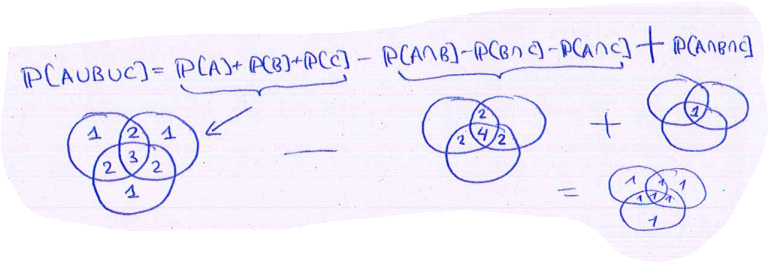
\includegraphics[width=0.8\textwidth]{img/sieb.PNG}\medskip\\
	\textbf{Für 4 Ereignisse A,B,C,D}\\
	$\mathds{P}[A]+\mathds{P}B+\mathds{P}[C]+\mathds{P}[D]$
	$-(\mathds{P}[A\cap B]+\mathds{P}[A\cap C ]+...+\mathds{P}[C\cap B]) $\smallskip
\\	$+ (\mathds{P}[A \cap B \cap C ] + \mathds{P}[B \cap C \cap D]+...)$
	$-\mathds{P}[A\cap B \cap C \cap D]$\medskip\\
	\textbf{Für n Ereignisse} $A_1,A_2,...,A_n$:\\
	$\mathds{P}[\bigcup^n_{k=1}A_k]=\Sigma^n_{i=1}\mathds{P}[A_i]-\Sigma_{1\leq i < j \leq n}\mathds{P}[A_i\cap A_j]+\Sigma_{1\leq i < j<k\leq n} \mathds{P}[A_i\cap A_j\cap A_k]- ... $\smallskip\\
	$+ (-1)^{n+1}\mathds{P}[A_1\cap ... \cap A_n]$\\\\
	\textbf{Beispiel:}\\
n Briefe werden zufällig in n adressierte Briefumschläge gesteckt.\medskip\\
Ereignis A = ''mind. 1 Brief wird in den richtigen Umschlag gesteckt''\medskip\\
$\mathds{P}[A] = ?$\medskip\\
\textbf{Lösung:}\\
Briefe 1,2,3,4,5,6\medskip\\
$\Omega = \{\underbrace{(a_1,...,a_i)}_{\substack{a_i\text{ gibt an, in welchen}\\\text{ Umschlag Brief i gesteckt wird}}}: a_i \in \{1,...,n\} a_i \neq a_j \forall i \neq j \}$\medskip\\
\#$\Omega = n*(n-1)*...+1=n! \quad \#A = ?$\\
A = \{$(a_1,...,a_n)\in \Omega: \exists k \text{ mit } A_k = k$\}\medskip\\
A = $A_1\cup ...\cup A_n$ mit \\
$A_k$ = ''Brief k wird in Umschlag k gesteckt''\medskip\\
$\mathds{P}[A_k] = \dfrac{\#A_k}{\#\Omega}=\dfrac{(n-1)!}{n!} = \dfrac{1}{n}$\smallskip\\
$A_1,...,A_n $ nicht disjunkt.\\
$\mathds{P}[A_1\cap A_2] = \dfrac{\#(A_1 \cap A_2)}{n!} = \dfrac{(n-2)!}{n!}$\medskip\\
$\mathds{P}[A_1\cap A_2\cap A_3]=\dfrac{\#(A_1 \cap A_2 \cap A_3)}{n!} = \dfrac{(n-3)!}{n!}$\medskip\\
\textbf{Allgemein}: $ \mathds{P}[A_{i1}\cap A_{i2}\cap...\cap A_{il}]=\dfrac{(n-l)!}{n!}$\smallskip\\
\textbf{Siebformel}: $\mathds{P}[A] = \mathds{P}[A_1\cup ... \cup A_n]= n * \frac{1}{n}- \binom{n}{2}*\dfrac{(n-2)!}{n!}+\dfrac{(n-3)!}{n!}-...$\medskip\\
$= \Sigma_{l=1}^n \binom{1}{l}*\dfrac{(n-l)!}{n!}*(-1)^{l+1}= \Sigma_{l=1+n}^n\dfrac{(-1)^{l+1}}{l!}$ \medskip\\
$=1-\dfrac{1}{2!}+\dfrac{1}{3!}-\dfrac{1}{4!}+...+(-1)^{n+1}\dfrac{1}{n!}$\medskip\\
Für $n\rightarrow\infty  \quad \underset{n\rightarrow\infty}{\text{lim}}\mathds{P}[A]= 1-\dfrac{1}{2!}+\dfrac{1}{3!}-\dfrac{1}{4!}+... $\smallskip\\
$= 1- (\dfrac{1}{2!}-\dfrac{1}{3!}+...)= 1 - \dfrac{1}{e} \approx 0.632$
